\chapter{Marco teórico}
\label{ch:marco}

\section{Descripción}

En un sistema de paneles fotovoltaicos es de suma importancia la eficiencia energética, para esto se debe estudiar el funcionamiento, curvas características, parámetros para poder caracterizar un panel, el modelo matemático tanto el ideal como la aproximación real, ecuaciones características obtenidas a partir de cada modelo, características del sistema que se requiere optimizar, algoritmos de calculo para realizar operaciones que se requieren en la solución, entre otros.

\section{Panel Fotovoltaico}

Las celdas solares se pueden describir como una junta \nt{p-n}, por medio de la radiación electromagnética proveniente del sol que incide sobre la capa de semiconductor, esta se transforma en el electricidad por un efecto fotovoltaico, en donde los fotones al tener mayor energía que la banda prohibida del semiconductor crean un par electrón-hueco, el campo eléctrico que se ejerce en la junta \nt{p-n} mueve los electrones (\nt{portadores}) lo que produce una fotocorriente, esta es directamente proporcional a la radiación del sol. Debido al proceso de fabricación del panel, posee un comportamiento exponencial y no lineal muy similar al de un diodo [1]. 

\subsection{Curvas Corriente-Tensión(I-V) para un PV }

\begin{figure}[H]
  \centering
    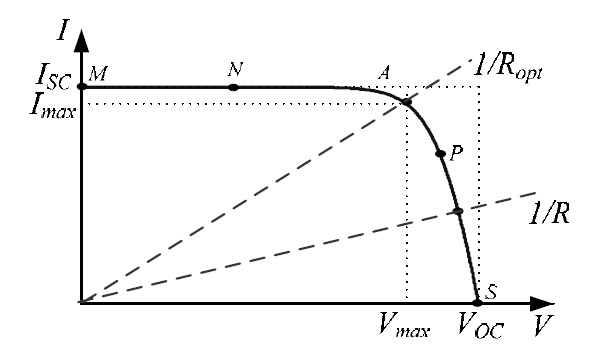
\includegraphics[scale=0.6]{./IV.jpg}
    \rule{35em}{0.5pt}
  \caption[Curva Corriente(A)-Tensión(V)]{Curva Corriente(A)-Tensión(V) }
  \label{fig:Curva_PV}
\end{figure}

La curva característica de un PV  se puede obtener manteniendo fijos los parámetros de irradiancia(S) y temperatura(T) esto bajo condiciones controladas, si se tiene una carga en las terminales de salida, la potencia entregada solo dependerá del valor de la carga, de manera que si la carga es pequeña (puntos M-N) el panel se comportará como una fuente de corriente, pero si la carga es grande(puntos PS) se comportará como una fuente de tension[2]. 

Dentro de la caracterización de la celda se realizan varias pruebas: 

\begin{compactitem}

\item \nt{Corriente de corto circuito $\ I_{sc}$ }: Se define como el valor máximo de la corriente generada por el panel, en condiciones de cortocircuito $\ V=0$.


\item \nt{Tensión de circuito abierto $\ V_{oc}$}: Se define como el valor que se tiene en la junta \nt{p-n} cuando se tiene una corriente generada $\ I=0$.

\item  \nt{Punto de máxima potencia}: se puede observar en el punto A$\left(V_{max},I_{max} \right)$ de la figura \ref{fig:Curva_PV} donde la potencia máxima de la carga resistiva es $\ P_{max} = V_{max}I_{max}$


\end{compactitem}



\subsection{Modelos del panel fotovoltaico}

Un panel fotovoltaico se puede modelar de manera simple (ideal), utilizando una fuente de corriente en paralelo con un diodo, la corriente de salida sera proporcional al radiación sobre la celda (foto-corriente)

\begin{figure}[H]
  \centering
    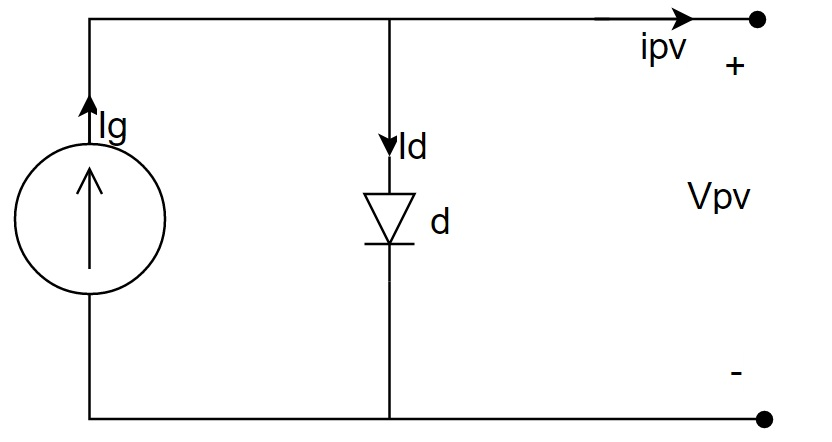
\includegraphics[scale=0.5]{./M1PV.jpg}
    \rule{35em}{0.5pt}
  \caption[Modelo simple ideal para un PV]{ Modelo simple ideal para un PV}
  \label{fig:Modelo1_PV}
\end{figure}

La figura \ref{fig:Modelo1_PV} muestra el modelo básico, sin embargo este se puede realizar de una manera mas compleja, agregando variables para las características del panel: 

\begin{compactitem}

\item Dependencia de la Temperatura, la corriente de saturación del diodo (\nt{Is}) y la foto corriente (\nt{Ig})


\item Perdidas debidas al flujo de corriente (\nt{Rs}) y perdidas con referencia a tierra (\nt{Rp}).

\item  Un parámetro \nt{n} que será el numero de celdas en análisis. 

\end{compactitem}

\begin{figure}[H]
  \centering
    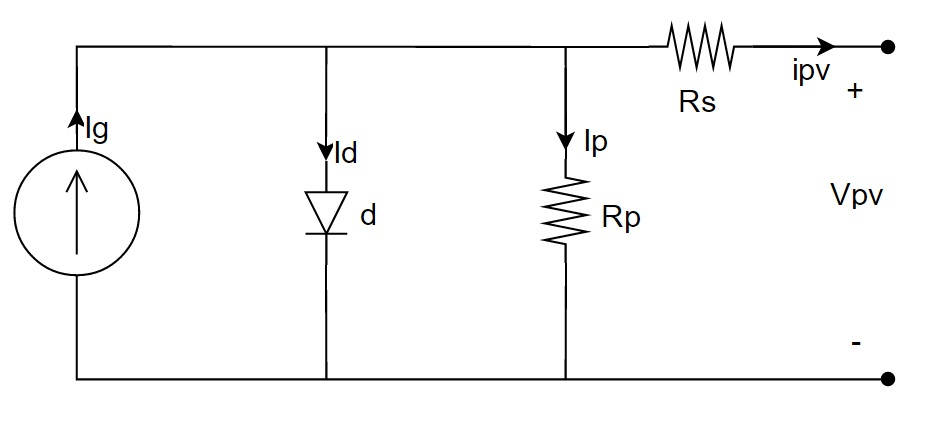
\includegraphics[scale=0.5]{./M2PV.jpg}
    \rule{35em}{0.5pt}
  \caption[Modelo con perdidas para un PV]{ Modelo con perdidas para un PV}
  \label{fig:Modelo2_PV}
\end{figure}

A partir del modelo con perdidas se puede deducir la ecuación que describe las corrientes, como sigue a continuación[4]:

\begin{equation} \label{eq:ej1}
  i_{pv}
  = I_{s} - i_{d} + i_{p}
\end{equation}

\begin{equation} \label{eq:ej2}
  I_{g}
  =
  2i_{pv} + \frac{V_{pv}+i_{pv}R_{s}}{R_p} -  I_{s} + I_{s}e^{ \frac{V_{pv}+i_{pv}V_{pv}}{n v_t}} 
\end{equation}

\textsl{Despejando $\ i_{pv}$}

\begin{equation} \label{eq:ej3}
  i_{pv} 
  =
  \frac{1}{2} \left[I_{s} + I_{g} - \frac{V_{pv}+i_{pv}R_{s}}{R_p} - I_{s}e^{ \frac{V_{pv}+i_{pv}V_{pv}}{n v_t}} \right]
\end{equation}
  
  
En general, la corriente que fluye por las terminales de un generador fotovoltaico está determinado por tres funciones de corriente:
\begin{compactitem}
\item \nt{Ig}: Corriente generada debido al efecto fotoeléctrico
\item \nt{id}: Corriente de pérdida debido a la juntura p-n
\item \nt{ip}: Corriente de pérdida de naturaleza resistiva
\end{compactitem}


 Para obtener un modelo del comportamiento estático del generador fotovoltaico se supondrá lo siguiente:

\begin{compactitem} 
\item \nt{Ig}: depende de la Irradiancia (S), pero no depende de la tensión en las terminales del generador fotovoltaico (\nt{Vpv})
\item \nt{ip} e \nt{id}: dependen de la tensión \nt{Vpv}
\item \nt{ip}: Depende de la temperatura (T)
\end{compactitem}

\textsl{De esta forma, la expresión que define $\ i_{pv}$}

\begin{equation} \label{eq:ej4}
  i_{pv} \left(V_{pv},T,S \right) 
  =
  i_g \left(V_{pv}\right)-i_d \left(V_{pv},T\right)
\end{equation}

\textsl{Según se definan las funciones $\ i_{pv}$ e $\ i_{d}$ se obtendrán modelos con complejidad y precisiones distintas, como los siguientes casos:  }


\begin{table}[H]
\centering
\caption{Modelos para un PV}
\label{Table:Modelos}
\begin{tabular}{|l|c|c|c|}
\hline
Modelos                                                             & $\ i_g$     & $\ i_p$ & $\ i_d$       \\ \hline
\begin{tabular}[c]{@{}c@{}} 1
\end{tabular}  & $\ KS $ & -   & $\ I_s\left(T\right)\left[e^\frac{V_{pv}}{v_t}-1\right] $          \\ \hline
\begin{tabular}[c]{@{}c@{}} 2
\end{tabular} & $\ KS $ & $\ G_pV_{pv} $   & $\ I_s\left(T\right)\left[e^\frac{V_{pv}}{v_t}-1\right] $          \\ \hline

\begin{tabular}[c]{@{}c@{}} 3 
\end{tabular} & $\ KS $ & -   & $\ I_s\left(T\right)\left[e^\frac{V_{pv} + i_{pv}R_{s} }{v_t}-1\right] $          \\ \hline
\begin{tabular}[c]{@{}l@{}} 4
\end{tabular} & $\ KS $ & $\ G_pV_{pv} + G_pi_{pv}R_s $   & $\ I_s\left(T\right)\left[e^\frac{V_{pv} + i_{pv}R_{s}}{v_t}-1\right] $     \\ \hline

\end{tabular}
\end{table}

De manera general se tiene: 

\begin{equation} \label{eq:ej5}
  i_{pv} \left(V_{pv}\right) 
  =
  G_{p}V_{pv} + G_{p}i_{pv}R_s
\end{equation}


\begin{equation} \label{eq:ej6}
  i_{d} \left(V_{pv}\right) 
  =
  I_s \left(T \right) e^\frac{V_{pv}}{v_t} e^\frac{ i_{pv}R_{s}}{v_t} -I_s \left(T \right)
\end{equation}

De esta forma el modelo general del comportamiento estático de un generador FV también se puede representar de la siguiente manera: 

\begin{equation} \label{eq:ej7}
  i_{pv}  
  =
  KS - G_{p}V_{pv} + I_s \left(T \right) - G_{p}i_{pv}R_s - I_s \left(T \right) e^\frac{V_{pv}}{v_t} e^\frac{ i_{pv}R_{s}}{v_t} 
\end{equation}

\begin{equation} \label{eq:ej8}
  I_s \left(T \right) e^\frac{V_{pv}}{v_t} e^\frac{ i_{pv}R_{s}}{v_t}   
  =
  KS - G_{p}V_{pv} + I_s \left(T \right) - G_{p}i_{pv}R_s - i_{pv} 
\end{equation}

La ecuación \ref{eq:ej8} es no lineal, aplicando una linealización, se tiene [3]: 

\begin{equation} \label{eq:ej9}
  y = ln \left(KS - G_{p}V_{pv} + I_s \left(T \right) - G_{p}i_{pv}R_s - i_{pv} \right) 
\end{equation}

si $ I_g = KS >> I_s $

\begin{equation} \label{eq:ej10}
  y = ln \left(KS - G_{p}V_{pv} - G_{p}i_{pv}R_s - i_{pv} \right) 
\end{equation}

\begin{equation} \label{eq:ej11}
  z = V_{pv} + i_{pv}R_s  
\end{equation}

posteriormente a un proceso de calculo de parámetros se tiene: 

\begin{equation} \label{eq:ej12}
  \theta_1  = ln\left( I_s \left(T \right) \right)
\end{equation}

\begin{equation} \label{eq:ej13}
  \theta_2  = \alpha 
\end{equation}

\section{Algoritmo de CORDIC}

El algoritmo \nt{Coordinate Rotational DIgital Computer} (CORDIC) es un método numérico en donde se realiza cierto numero de iteraciones para encontrar el valor deseado según sea la función en calculo, este algoritmo es utilizado para implementar funciones trigonométricas, logarítmicas y  exponenciales. La facilidad de implementación, hace que sea uno de los algoritmos mas utilizados en el ámbito de la electrónica digital, CORDIC utiliza desplazamientos, sumas, restas y tablas look-up con valores previamente precargados en una memoria ROM, estos valores dependerán de la operación en calculo, se puede utilizar el método circular, lineal e hiperbólico.   

Las ecuaciones generales para el algoritmo de CORDIC se definen como: 

\begin{equation} \label{eq:ej14}
  X_{i+1} = X_{i}- md_{i} 2^{-i} Y_{i}  
\end{equation}

\begin{equation} \label{eq:ej15}
  Y_{i+1} = Y_{i}- d_{i} 2^{-i} X_{i}  
\end{equation}

\begin{equation} \label{eq:ej16}
  Z_{i+1} = Z_{i}- d_{i} e\left(i\right)
\end{equation}

donde $\ e\left(i\right) $ se muestra en la tabla \ref{Table:ei} [5] según sea el caso:

\begin{table}[H]
\centering
\caption{Sistema de coordenadas unificado (CORDIC)}
\label{Table:ei}
\begin{tabular}{|l|c|c|c|}
\hline
m & Sistema de coordenadas                                                             & Valor de $\ e\left(i\right) $     \\ \hline
\begin{tabular}[c]{@{}c@{}} 1
\end{tabular}  & Circular & $\ tan^{-1}\left(2^{-i}\right)$         \\ \hline
\begin{tabular}[c]{@{}c@{}} 0
\end{tabular} & Lineal & $\ 2^{-1} $          \\ \hline

\begin{tabular}[c]{@{}c@{}} -1 
\end{tabular} & Hiperbólico & $\ tanh^{-1}\left(2^{-i}\right)$                \\ \hline


\end{tabular}
\end{table}



\subsection{Sistema de coordenadas hiperbólico}

Para el calculo de algunas funciones que no son tan directas con el algoritmo, se utilizan identidades [6] para el calculo como sigue:

\begin{equation} \label{eq:ej17}
  \tan z = \frac{\sin z}{\cos z}
\end{equation}

\begin{equation} \label{eq:ej18}
  \tanh z = \frac{\sinh z}{\cosh z}
\end{equation}

\begin{equation} \label{eq:ej19}
  \exp z = \sinh z + \cosh z
\end{equation}

\begin{equation} \label{eq:ej20}
  \ln \omega = 2 \tanh^{-1} \left( \frac{y}{x} \right)
\end{equation}

donde: 

\begin{equation} \label{eq:ej21}
  x = \omega + 1
\end{equation}

\begin{equation} \label{eq:ej22}
  y = \omega - 1
\end{equation}

\subsection{Logaritmo natural utilizando el algoritmo hiperbólico de CORDIC}
Para un $\ Ln \left(\omega\right) $  con el algoritmo de CORDIC, se debe calcular primeramente la $\ \tanh^{-1} \left( \frac{y}{x} \right)$ con las siguientes ecuaciones:

 
\begin{equation} \label{eq:ej23}
  X_{i+1} = X_{i} + d_{i} 2^{-i} Y_{i}  
\end{equation}

\begin{equation} \label{eq:ej24}
  Y_{i+1} = Y_{i} + d_{i} 2^{-i} X_{i}  
\end{equation}

\begin{equation} \label{eq:ej25}
  Z_{i+1} = Z_{i} - d_{i} tanh^{-1}\left(2^{-i}\right)
\end{equation}

donde $\ i $ es el indice de cada iteración, las iteraciones 4, 13, 40,… k, 3k+1 se deberán repetir para garantizar la convergencia. $\ d_i $ es el signo de $\ Y_i $ invertido, es decir el cuando el signo de $\ Y_i $ es negativo, $\ d_i $ será positivo y viceversa.

Utilizando la ecuación \ref{eq:ej20} se definen los valores de entrada para las ecuaciones anteriores  $\ X_0 = \omega + 1$ , $\ Y_0 = \omega - 1$ y $\ Z_0 = 0 $.

Cabe destacar que el rango de convergencia para este algoritmo [7] se puede definir como: 

\begin{equation} \label{eq:ej26}
   0.106843 \leq \omega \leq 9.35947
\end{equation}

donde $\ \omega $ es el valor del argumento del logaritmo natural.

El resultado final de $\ Z_i $ contiene el valor de $\ \tanh^{-1} \left( \frac{y}{x} \right)$, sin embargo se debe multiplicar por un factor de 2 para completar el calculo del logaritmo natural, segun la identidad de la ecuación \ref{eq:ej20} 

\subsection{Exponencial utilizando el algoritmo hiperbólico de CORDIC }


Para una función  $\ e^{\left(\omega\right)} $  con el algoritmo de CORDIC, se debe utilizar las ecuaciones \ref{eq:ej23}, \ref{eq:ej24} y \ref{eq:ej25} de manera iterativa, donde el valor final de $\ X $ y $\ Y$, son el resultado para  $\\cosh\left(\omega\right)$ y $\ \sinh\left(\omega\right)$ respectivamente. se debe tomar en cuenta la repeticion de las iteraciones $\ \left(i\right) $ 4, 13, 40,… k, 3k+1 para garantizar la convergencia dando una mejor precision en el calculo.

Los valores iniciales se definen como \nt{constantes} $\ X_0 = 1.20753406 $ , $\ Y_0 = 0$ y $\ Z_0 = \omega $ donde $\ \omega$  es el valor del argumento que se desea calcular y $\ d_i $ es el signo de $\ Z_i $.

Cabe destacar que el rango de convergencia para este algoritmo se puede definir como: 

\begin{equation} \label{eq:ej26}
   0 \leq \omega \leq 1
\end{equation}

El valor final del calculo se obtiene mediante una suma con la identidad de la ecuación \ref{eq:ej19}. 

\section{Punto flotante}
La codificación para el formato punto flotante se realiza mediante el estándar \nt{IEEE 754}, este requiere de tres campos en la palabra: 

\begin{compactitem}
\item Signo 
\item Exponente
\item Mantisa 
\end{compactitem}

para el formato \nt{IEEE 754} de 32-bits [8] se asigna: 

\begin{compactitem}
\item 1 Bit para signo 
\item 8 Bits para exponente
\item 23 Bits para mantisa 
\end{compactitem}

Donde el bit de signo representa un numero positivo si este es 0, de manera contraria si es 1 representa un numero negativo. 

El exponente puede representar 256 (8-bits) valores sin embargo se tiene:

\begin{compactitem}
\item $\ \left[0-127\right]$ exponentes negativos  
\item $\ \left[128-255\right]$ exponentes positivos
\end{compactitem}

De esta manera para convertir el un exponente positivo en el valor correspondiente en punto flotante se debe sumar el valor del exponente como sigue $\ exp_{float}=127+exp $ , por otro lado si se desea pasar de un valor decimal a punto flotante se deben realizar los siguientes pasos: 
\begin{compactitem}
\item Representar el signo con su debido bit
\item Conversión decimal a binario punto fijo   
\item Conversión binario a notación científica
\item Agrupar en signo, exponente y mantisa 
\end{compactitem}



 
\section{Referencias bibliográficas}

[1] Suskis, Pavels, and Ilya Galkin. "Enhanced photovoltaic panel model for MATLAB-simulink environment considering solar cell junction capacitance." Industrial Electronics Society, IECON 2013-39th Annual Conference of the IEEE. IEEE, 2013.

[2] González-Longatt, Francisco M. "Model of photovoltaic module in Matlab." II CIBELEC 2005 (2005): 1-5.

[3] C. Meza, R. Ortega, "Control and estimation scheme for PV central inventers", in 24th International Conference on information, Comunication and Automation Technologies, Nov, 2013 

[4] Chiang, Ching-Tsan, Tung-Sheng Chiang, and Hou-Sheng Huang. "Modeling a photovoltaic power system by CMAC-GBF." Photovoltaic Energy Conversion, 2003. Proceedings of 3rd World Conference on. Vol. 3. IEEE, 2003.

[5] Ibrahim, Muhammad Nasir, et al. "Hardware Implementation of Math Module Based on CORDIC Algorithm Using FPGA." Parallel and Distributed Systems (ICPADS), 2013 International Conference on. IEEE, 2013.

[6] Walther, John S. "A unified algorithm for elementary functions." Proceedings of the May 18-20, 1971, spring joint computer conference. ACM, 1971.

[7] Llamocca-Obregón, Daniel R., and Carla P. Agurto-Ríos. "A fixed-point implementation of the expanded hyperbolic CORDIC algorithm." Latin American applied research 37.1 (2007): 83-91.

[8] Whitehead, Nathan, and Alex Fit-Florea. "Precision and performance: Floating point and IEEE 754 compliance for NVIDIA GPUs." rn (A+ B) 21 (2011): 1-1874919424.



